% 来源：OEBPS/Text/Section0001_split_002.xhtml#sigil_toc_id_19

\BookChapter{10}
\section[第10章\q 投资营销谎言5：“退休金有401(k)就行”]{第10章\\ 投资营销谎言5：“退休金有401(k)就行”}

\begin{BookQuote}
401(k)计划是个退休养老金大实验，婴儿潮世代成了最早的一批小白鼠。

\hfill ——道格·沃伦（《协同效应》作者）
\end{BookQuote}

很多想法和发明创造一开始都有良好的意愿。核聚变打开了人类免费使用能源的大门，现在可以为整个城市提供电力。但是如果把核聚变装进一个导弹，导弹就可以把整个城市夷为平地。

经常使用一点人类的贪婪和聪明才智，我们就可以把某些伟大的好事转化成能够带来坏处多于好处的坏事，例如401(k)计划本来只是一条小小的免税代码，代表雇员部分收入可以免税。如果正确运用，它可以加快我们的退休金积累，让我们能够提前几年退休。但是如果像今天大多数的401(k)计划被那样运用的话，它会破坏我们实现财务自由的机会。

因为401(k)账户可能是大多数人拥有的唯一一个退休金账户，所以这章可能是本书最重要的一章。下面我们会展示给大家如何运用401(k)计划，而不是让这个计划来支配你，你会发现如何贯彻实施我们前面所学的大部分东西，好让401(k)计划成为对于你来说非常棒的退休金计划，而不是成为银行理财经理、券商经纪人或者公募基金经理的一个退休金积累计划。但是，首先了解一些背景故事非常重要。

\subsection{401(k)计划是如何发展成现在这个样子的？}

1984年推出的401(k)计划给我们提供了参与股票市场的机会。通过拥有美国市场经济体系的一小部分，企业雇员养老金计划可以节省纳税开支，因为把一部分工资收入储蓄到这个养老金账户，可以在税前扣减应纳税所得额。

但是401(k)计划从来没有打算成为美国人唯一的养老金计划。为此，我请教了约翰·肖文，他是斯坦福大学的经济学教授。我们在电话交流时，他说得非常清楚：“托尼，你不可能指望连续30年把储蓄收入的3\%储蓄起来，然后就指望着靠这笔钱在退休之后享有和你在工作时完全相同的收入水平，再活上30年。”

我们不要忘了这个社会实验也不过几十年的历史，我们现在才开始看到一代人中的大多数要退休了，他们是唯一使用了401(k)计划的一代人。

我们回顾历史发现，401(k)计划开始时就是钻了一个法律的空子，目的是让那些收入很高的企业高管能够储蓄更多的钱。后来，它成了整个公司的一种福利，公司决定用它来消除传统养老金让公司承担的成本和义务，把所有的风险和费用都转移到雇员个人身上。这并不是说原来的养老金体制本身没有问题，例如，你换了工作，但你交的养老金不能跟着你换到新的公司。

有意思的是，企业雇员并不在意承担这种新的责任，因为那个时候股市正在猛涨，那些非常无聊的有保障的养老金，哪里比得上投资股票让自己更快速地发财致富？

于是资金流进了股市，远远超过了历史水平。所有这些新的资金意味着大量的购买，这正是推动20世纪八九十年代大牛市的燃料。眼前有数万亿美元唾手可得，公募基金公司开始了一场前所未有的战争，抢着要管理你的资金。股票市场不再仅是一个公司发行股票、上市的地方，上市公司可以用股权来交换现金。股市也不再只是一个只有高净值客户和经验老到的机构才会来投资的地方，股市成了每个人储蓄的工具。

\subsection{欢迎你，船长}

401(k)计划出现的时候代表着自由，而自由往往给我们一种控制的错觉。在股市上涨的时候，我们有时会错误地把运气好误认为自己“投资水平高”。

艾丽西亚·穆勒博士是波士顿学院退休研究中心的主任，是美国顶尖的退休养老问题研究专家。我们交谈了近两个小时，讨论了绝大多数美国人面临的退休养老危机。按照他的观点，我们原来实施的是固定福利养老金体制——每个人都有一份养老金，它是终身收入——现在换成了401(k)计划。对于雇主来说，很明显，401(k)计划使其负担轻多了；从表面上看，401(k)计划对个人也有利，因为雇员自己可以更多地控制自己的投资决策。但是即使是身为美国联邦储备局的前雇员和美国总统经济顾问委员会成员的艾丽西亚，在处理自己的养老金问题时，有些关键的步骤也走错了。所以，我现在有一个固定福利计划和终身收入保障是波士顿联邦储备银行作为雇主给我的。当我在财政部工作的时候，我的一位同事说，你早点把那些退休金拿出来吧，你自己用这些钱来做投资，要比联邦储备银行做的投资收益好得多。现在那些钱早就亏得无影无踪了。

自己对自己的投资决策负责，对于大多数人来说，他们一想到它就觉得很害怕。特别是在阅读本书之前，作为你自己的财务大船的船长，你必须在所有可以得到的投资选择中航行，并产生丰厚的收益，这样才足以支撑你的退休生活的开支。你要成为一个坚持利用部分时间投资的投资专家，同时还要做好你的全职工作，或者经营好自己的私人企业，以养家糊口。

特蕾莎·吉拉杜奇在纽约社会研究新学院工作。她在《纽约时报》上发表了一篇非常出色的文章《我们非常荒谬可笑的退休养老途径》。在这篇文章里，她只用一段话就罗列出了我们面对的所有挑战：

你还不相信现在的企业养老金计划，由雇员自愿选择，自我指导，商业化运营，其本身是存在缺陷，肯定会失败的吗？你好好想想，要让这套体系对你有效，需要具备哪些条件？第一，想清楚，什么时候你和你的配偶让雇主辞退了，或者生病了不能继续工作呢？第二，想清楚，什么时候你会死？第三，你要明白，你需要把自己挣的每一分钱都拿出来7\%用于储蓄。（要是25岁的时候，你没有开始这样储蓄，现在你55岁了，该怎么办？你现在挣到的每一分钱都要拿出来30\%储蓄起来才行。）第四，你的投资每年的收益率至少比通货膨胀率高出3\%。（这也容易。只要能找到最好的基金，用最低的价格买入，把这些基金做最优化的配置，你就能够做到。）第五，绝对不要从你的养老金里面提款，即使是丢了工作，健康出了问题，离婚了，买房了，送小孩上大学了，你也一分钱不要提。第六，安排好你的养老金账户提款的时间计划，好让你死的那一天正好花光养老金的最后一分钱。

是的，这套体系是需要时间的，也需要美国国会和华尔街方面取得很大的进展。但是好消息是，对于那些消息灵通、见多识广的人来说，他们能够驾驭好自己的退休养老金计划。你也可以像个内行那样运用好这套体系，让它为你的工作带来好处。

\subsection{再来一次吗？}

那么先让我们来回顾一下，我们现在已经知道了那些想要通过选股战胜市场的主动管理型公募基金并不能战胜市场。大多数401(k)计划购买的公募基金也是如此。我们也知道，这些费用高昂的公募基金收取天价般的费用会吃掉我们投资收益的50\%\textasciitilde{}70\%，具体比例取决于你现在的年龄。想一想，就在此时此刻公募基金通过收费拿走了你多少钱？1万美元？2.5万美元？10万美元？算一算吧，你把自己吓坏了吧？

那些收费昂贵的公募基金包含在一个知名的401(k)计划里面，这通常由薪酬外包服务公司或者保险公司向你提供。你一直持有这些公募基金，它们就会向你征收一大堆额外的费用。所有这些成本加在一起就会形成一道让你难以克服的障碍。使用绝大部分机构管理的养老金计划，会让你赢得401(k)计划这一游戏比赛的概率大大减小，甚至为零。

\begin{figure}[htbp]
\centering
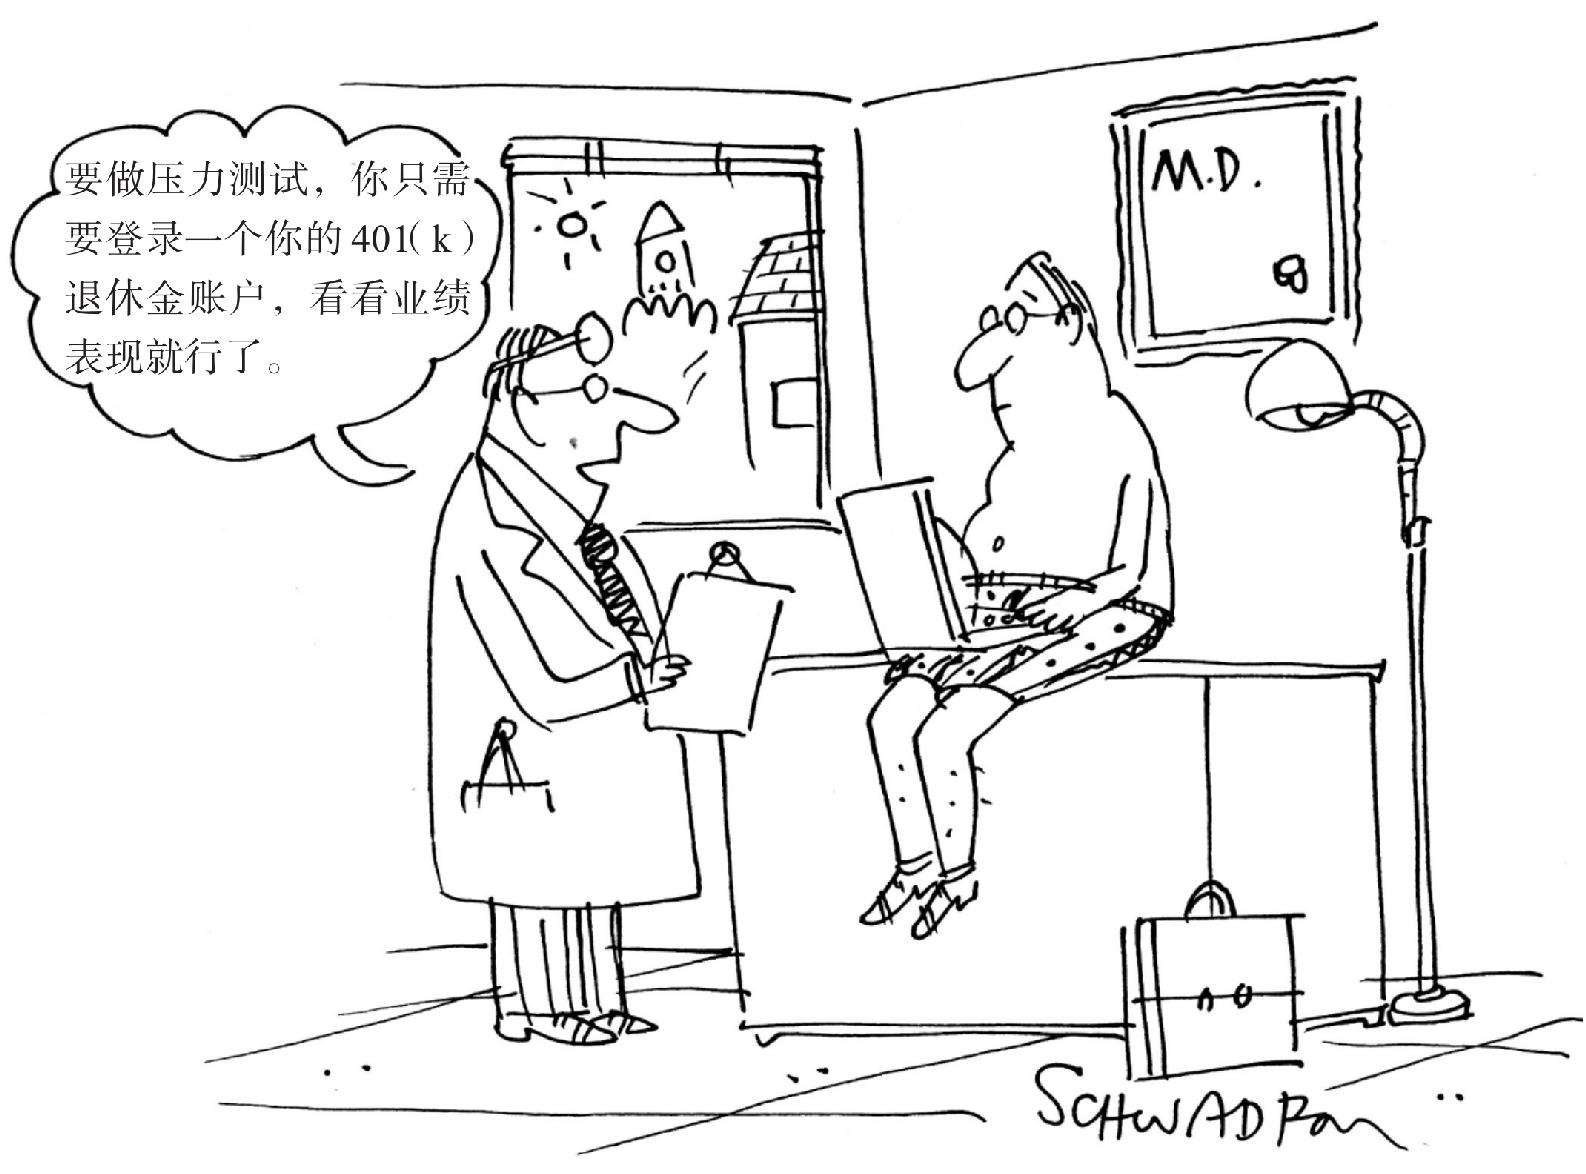
\includegraphics[width=0.78\linewidth,keepaspectratio]{image/10-1.jpg}
\caption{}\label{fig:10-1}
\end{figure}

401(k)计划可以得到延迟纳税的优惠，但是大多数人都需要支付19种不同的费用，用于投资管理和计划管理。

\subsection{沟通费用}

\begin{itemize}
\item 登记
\item 持续
\item 入会（会议）
\item 投资建议
\end{itemize}

\subsection{保存记录和行政管理费用}

\begin{itemize}
\item 基本费用
\item 每个参与者收费
\item 每个合格雇员收费
\item 分销费
\item 贷款发放
\item 贷款维护
\item 半年度审计测试
\item 5500个文档包
\item 其他费用
\end{itemize}

\subsection{投资费用}

\begin{itemize}
\item 基本费用
\item 个人（共同）基金费用
\item 经理/顾问费
\item 其他资产费用（收入共享、打包、行政管理，等等）
\end{itemize}

\subsection{托管费}

\begin{itemize}
\item 基本费用
\item 按人收费
\item 按资产收费
\end{itemize}

但是现在好了，你选了优质的401(k)计划，管理人的效率很高，花钱节省，不会拿走你的钱。这样你就可以把逆风变成顺风，利用政府赋予我们的优势，让自己获得更大的前进动力。

\subsection{美国最好401(k)？证明给我看！}

我真正明白了约翰·博格所说的成本复利效应的暴政，意识到了过高费用的毁灭性力量。我马上打电话给我公司的人力资源部的负责人，想要看一看我们自己公司的401(k)计划的具体情况。我想知道，我像关心自己家人一样关心他们是不是也正在被人洗劫一空。可以确定的是，我们使用的也是成本很高的名牌计划，里面都是收费很高的公募基金，还要收取过多的行政管理费用和经纪人费用。那个经纪人（相当于中国的银行理财经理）向我保证这个退休金计划是最顶尖的，收费低，路子正。确实是这样的，这个计划正好使他能赚钱付他新买的宝马车的月供。

我相信肯定会有更好的退休金计划，我和我的团队开始做一些研究工作，我们看了一大堆垃圾一样的退休金计划，这个过程令我们感到十分沮丧。我的一个好朋友提醒我，有一家公司的名字就叫美国最好401(k)。敢给公司起这样的名字，胆子真大。我打电话给这家公司的老板汤姆·兹甘乐，我说：“证明给我看。”

我们俩见面只谈了5分钟，我就发现，很明显，这个家伙很有激情，非常想要帮助人们摆脱那些设计非常糟糕、收费又非常多的401(k)计划。他说，401(k)计划行业是“美国最脏的资金池，因为没有人知道是谁，以及它是如何让人用钱收买了的。”他竟然给自己从事的行业做出如此糟糕的评价！“老兄，你要知道，这个行业才有30年的历史。到2012年，这个行业才有了法律法规，才要求服务提供商公开披露费用。但是尽管披露了费用，所有雇员中超过一半的人还不知道他们现在付的费用到底有多高。”其实参与401(k)计划的人里面，有67\%的人认为根本没有费用。当然，再没有什么其他想法比这更偏离事实真相了。

“汤姆，那么你和你的同行有什么不同？你给自己的公司起名为美国最好401(k)，你凭什么说你的公司是美国最佳呢？”上当受骗过之后，我现在非常小心谨慎，就像小熊爸爸照顾自己的熊孩子一样，因为我知道我的这个决定将会直接影响到我的雇员和他们的孩子。多年来，他们一直在支付过多的费用，我不能允许这种事再次发生。我已经想明白了，作为公司的老板，我既是企业的主人，也是401(k)计划的赞助人，我的法律义务就是要确保我的雇员没有让别人占便宜。（后面我会详述。）

汤姆解释说：“老兄，我们公司的名字就叫美国最好401(k)，我们只允许成本极低的指数基金被纳入计划，比如先锋公司和三维基金公司，而且我们不会因为销售公募基金从基金公司手里拿到一分钱的回扣。”我刚刚采访了约翰·博格，他确认了先锋公司不参与任何花钱才能玩的游戏，这是公募基金的普遍做法，只有如此，它才能参与401(k)计划，从中分到一笔收入。顺便说一下，对于你来说，这意味着你在401(k)计划中的基金选择，并非你能得到的最好的基金选择。那些基金公司都是花了大价钱，才能被列入选择名单的。你猜猜这些基金公司为了进入基金选择名单花了大钱，它们怎么捞回来这些成本？当然是利用高收费了。所以不但你不能得到业绩最好的基金，而且你往往为了业绩更差的基金付出了更高的费用。

“我明白了，汤姆。那么其他计划的费用还有哪些？我想要看看每一笔可能发生的费用。我要完整披露，要完全透明，一笔也不能少！”

汤姆非常骄傲地拿出来一张带有编号的费用一览表，隔着桌子递给了我：“所有的成本，包括投资选择、投资管理服务、保存记录费用。所有的成本费用加起来，每年只有0.75\%。”

“就只有这么多吗？没有隐藏费用吗？或者没有不知什么时候会冒出来的其他费用吗？”

我们把全部成本费用从超过2.5\%减少到只有0.75\%，减少了70\%。你可以回忆一下我们在第2章中讲过的复利效应，经过一段时间，在复利的作用下，这些费用会积少成多，达到上万美元甚至上百万美元——现在这么多钱会重新回到我的雇员和他们家人的手中。这让我感觉好极了。下面就是一张简单的对比图，一个是样板401(k)计划，类似于我们公司过去一直用的那一种，另一个是美国最好401(k)计划。将二者进行对比，你可以看到，这些节省下来的费用按照复利计算会有多少钱直接返回到我的雇员的养老金账户里。

% 来源：OEBPS/Text/Section0001_split_002.xhtml → image_edbab4e9a7d44b9990a55ef2df9511d6.jpg
\begin{longtable}{@{}C{\dimexpr 0.13000\linewidth-1.50000\tabcolsep\relax}C{\dimexpr 0.29000\linewidth-1.50000\tabcolsep\relax}C{\dimexpr 0.29000\linewidth-1.50000\tabcolsep\relax}C{\dimexpr 0.29000\linewidth-1.50000\tabcolsep\relax}@{}}
\caption{美国最好401(k)公司的退休金计划}\label{tab:10-1}\\
\toprule\noalign{\vskip 3pt}
{\heiti 时间} & {\heiti 我原来的计划（总费用的2.5\%）} & {\heiti 美国最好公司的401(k)退休计划} & {\heiti 返回到你和你雇员账户的总存款} \\
\midrule
\endfirsthead
\multicolumn{4}{r}{续表}\\[0.6em]
\toprule\noalign{\vskip 3pt}
{\heiti 时间} & {\heiti 我原来的计划（总费用的2.5\%）} & {\heiti 美国最好公司的401(k)退休计划} & {\heiti 返回到你和你雇员账户的总存款} \\
\midrule
\endhead
\bottomrule
\endfoot
\bottomrule
\multicolumn{4}{@{}p{\linewidth}@{}}{\footnotesize 单位：美元。}\\
\endlastfoot
1年后\footnote{\label{fn:table-表10-1-1}假设一开始账户余额为100万美元，每年存入10万美元，每年增长率为5\%} & 15\,925\,465 & 16\,006\,101 & 80\,635 \\
7年后 & 22\,265\,866 & 23\,025\,978 & 760\,111 \\
20年后 & 41\,999\,917 & 45\,999\,618 & 39\,999\,701 \\
\end{longtable}


% 来源：OEBPS/Text/Section0001_split_002.xhtml → image_cb61ac24d2b340e3943f40fd0de38da4.jpg
\begin{longtable}{@{}C{\dimexpr 0.13000\linewidth-1.50000\tabcolsep\relax}C{\dimexpr 0.29000\linewidth-1.50000\tabcolsep\relax}C{\dimexpr 0.29000\linewidth-1.50000\tabcolsep\relax}C{\dimexpr 0.29000\linewidth-1.50000\tabcolsep\relax}@{}}
\caption{美国最好401(k)公司的退休金计划}\label{tab:10-2}\\
\toprule\noalign{\vskip 3pt}
{\heiti 时间} & {\heiti 我原来的计划（总费用的2.5\%）} & {\heiti 美国最好公司提供的401(k)退休金计划} & {\heiti 返回到你和你雇员账户的总存款} \\
\midrule
\endfirsthead
\multicolumn{4}{r}{续表}\\[0.6em]
\toprule\noalign{\vskip 3pt}
{\heiti 时间} & {\heiti 我原来的计划（总费用的2.5\%）} & {\heiti 美国最好公司提供的401(k)退休金计划} & {\heiti 返回到你和你雇员账户的总存款} \\
\midrule
\endhead
\bottomrule
\endfoot
\bottomrule
\multicolumn{4}{@{}p{\linewidth}@{}}{\footnotesize 单位：美元。}\\
\endlastfoot
1年后 & 14\,530\,987 & 14\,582\,411 & 51\,424 \\
7年后 & 25\,077\,485 & 25\,623\,388 & 546\,899 \\
20年后 & 58\,499\,799 & 61\,756\,687 & 3\,355\,987 \\
\end{longtable}


让超过120万美元重新回到我的家人和雇员手里，我们只做了一个简单的转换就实现了。顺便说一下，这个计算只考虑了费用，没有考虑我们的基金业绩战胜了96\%的公募基金经理。因为我们使用的是低成本的模仿市场的指数基金。

\subsection{扩音器}

汤姆和他的团队为我们公司提供了新的401(k)计划，让我和我的雇员印象非常深刻。过了六个月后，我向我所有的朋友都推荐了汤姆和他的公司。我决定和美国最好401(k)公司合作，帮助它宣传推广。我知道我在本书里一定要讲这个故事，因为这家公司的收费实在太低了，所以它无法承担在超级碗上做广告的巨额费用。汤姆的这种草根做法正在不断地获得支持，我希望能够扩大他公司的知名度和影响力。

\subsection{现在是时候拉下窗帘了}

汤姆和他的团队搞了一个非常强大的在线费用检查器，它可以分析你们公司的雇员养老金计划的数据（从公司的纳税收入报表中）。只用几秒钟，你们公司的养老金计划和别的公司的对比情况，以及你实际上支付的费用，就可以显示出来。就像上面的表格，这个检查器也会显示长时间节省成本对于你来说意味着什么。如果你发现某计划可能给你节省上万美元，这并不是什么稀罕事。

\subsection{需要额外的激励吗？}

只是知道高昂的费用摧毁了你的养老金还不够，企业老板也会非常关心雇员应该“武装到牙齿”。为什么？因为美国劳工部出手了，要保护企业雇员，对抗费用高昂的养老金计划。谁应该负责任？企业老板！对。不是公募基金经理，不是经纪人，不是银行理财经理，也不是糟糕的401(k)计划管理人，而是企业老板会深深地陷入困境。

根据《首席财务官月报》的报道，2013年，美国劳工部审查了企业401(k)计划，75\%的企业赞助人因为计划出错而遭到罚款和处罚，或者被强迫做出补偿。这些罚款和处罚的费用可不是小数目。事实上，2013年平均每个计划的罚金是60万美元，比4年前增长了近15万美元。

而且美国劳工部在2014年就新增雇用了1000名执法人员。所以我们完全可以预期401(k)计划审查范围会进一步扩大，我不知道你怎么看，但是这确实让我十分关注。

感谢那些集体诉讼律师，现在很多公司正在被自己的雇员起诉，包括卡特彼勒公司、通用动力公司、美国银行，甚至是富达投资集团——行业内规模最大的401(k)计划供应商。最近，富达投资集团对两起集体诉讼案达成了和解，支付了1200万美元，起因是富达投资集团的雇员起诉公司的401(k)计划的费用过高。当然，这些大企业尽管亏了很多钱，但也亏得起。其实真正危险的是那些规模较小的企业老板，因为中小企业的401(k)计划规模更小（一般计划内的资产少于1000万美元），但费用是最高的。

那么，你作为企业老板应该做些什么？第一，你每年要把你的企业的养老金计划与其他企业的计划进行对比，这可是法律要求。新的法律从2012年才开始实施，所以对于你来说这可能还是新闻呢。美国劳工部要求，你要把你们企业的养老金计划与其他企业“有可比性的”计划进行对比，以确认你们企业的养老金计划的收费是合理的。我问过其他企业老板，他们都表示一无所知。我自己原来也是毫不知情。你想，那个把收费昂贵的养老金计划卖给你的家伙，他会打电话告诉你这件事吗？当然不会了。

\begin{figure}[htbp]
\centering
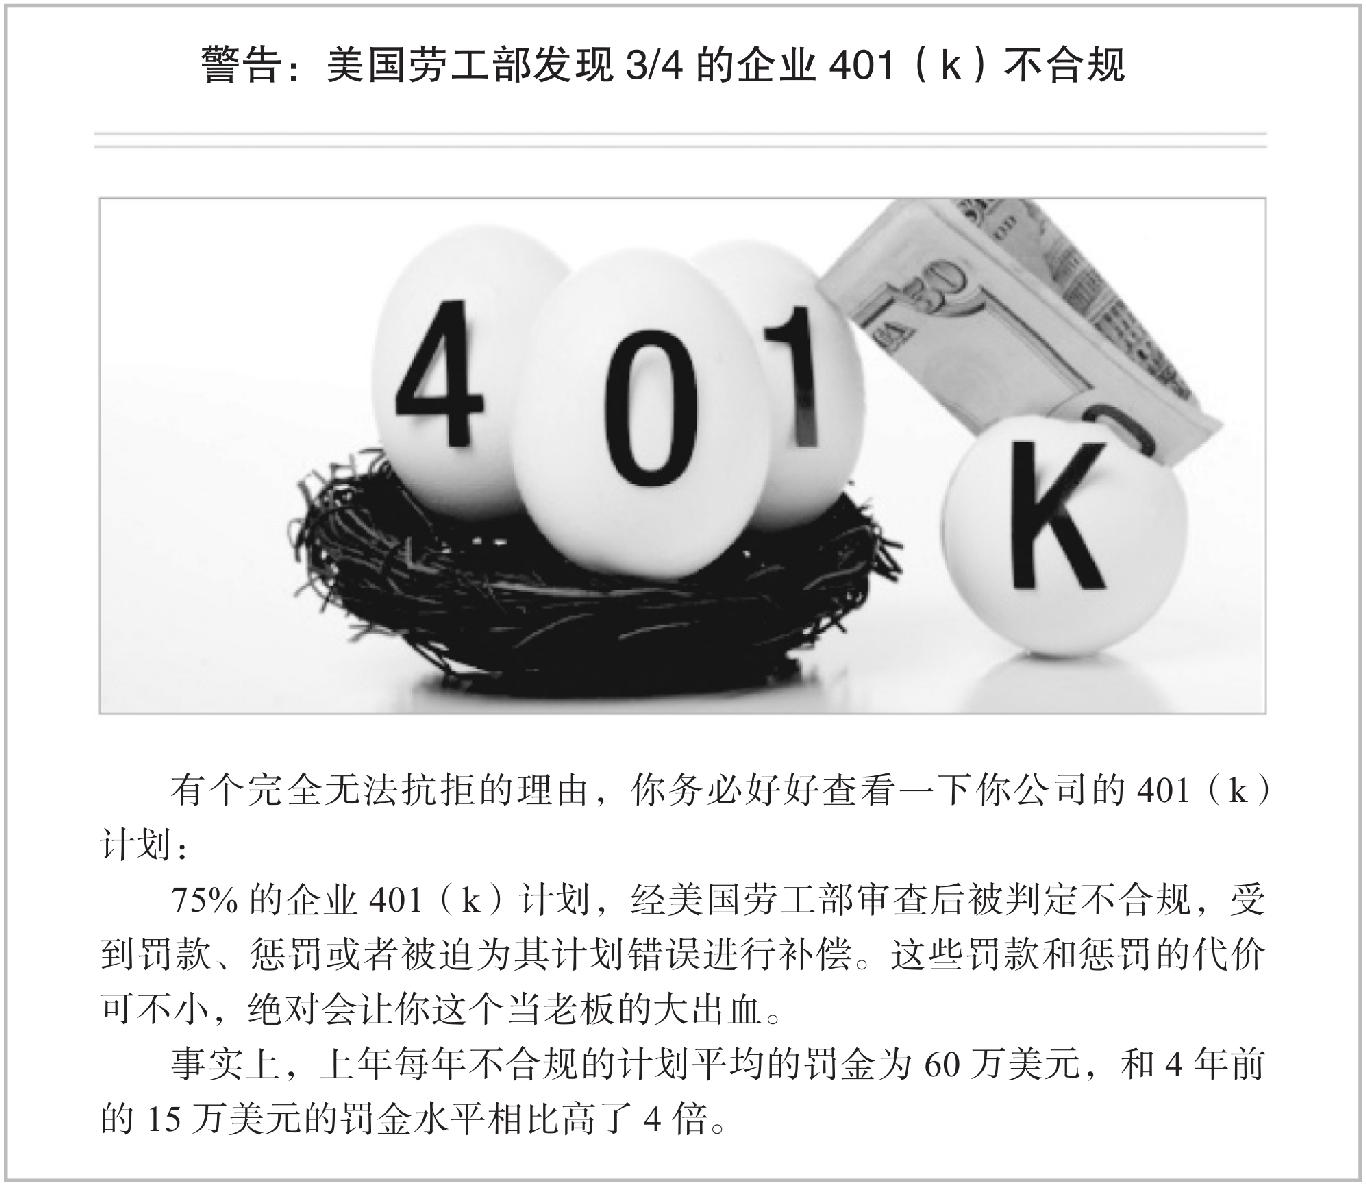
\includegraphics[width=0.86\linewidth,keepaspectratio]{image/10-2.jpg}
\caption{}\label{fig:10-2}
\end{figure}

美国最好401(k)计划不仅会提供给你完全免费的分析，而且会提供给你免费的对比基准。如果美国劳工部的检查人员在星期五的下午走进你的办公室，不要让他毁了你的周末，因为检查人员要检查的东西你没有准备好，你非常害怕地站在那里，像一只在晚上站在车灯前的小鹿一样，内心怦怦乱跳。你肯定希望自己能够自信地信手拿出你的企业养老金计划的对比基准。

\subsection{谁来悬崖勒马}

美国劳工部横冲直撞地进行大规模检查，会严厉地处罚企业老板。我一点儿也不知道，作为企业老板和养老金计划的出资人，我也是401(k)计划的法定受托人。有无数的案例表明，企业老板个人要为自己企业糟糕的401(k)计划负责。如果你用的401(k)计划是像美国最好401(k)这样的公司，那么它会给你“安排”一个专业的受托人，这会大幅度减轻你的法律责任（是的，这种服务也包括在每年0.75\%的费用里，不用另外付费），而且它会提供服务，帮你不断地进行对比检查——这是一项免费服务。

你如果是一个雇员，应该做什么呢？首先访问美国最好401(k)公司网站，用上面的费用检查器，检查你的401(k)计划的费用情况，然后把检查报告发送给你的老板（或者你的上级）。事实上，企业里收入最高的人，往往他的401(k)账户余额也是最高的。所以收费越高，这些高管的损失越大。其实你这样教育公司高管做好自己的401(k)计划，是给整个公司做了一件大好事。过高的费用会吸走每一个人辛辛苦苦挣的钱。适当改变一下，会大大增加每个人获得财务自由的机会。记住，我们每个人需要的都是顺风顺水，加速前进，而不是逆风逆水，阻挡我们前行。

你也可以直接走到公司的人力资源部，让他们好好读一下本章内容，并确定他们读懂了。如果费用不是一个激励因素，那么你要提醒他们，他们是你的受托人，你的同事，他们在法律上有义务向你确认他们有一个相当有竞争力的计划，而且要符合你的最大利益。这肯定能够吸引他们的注意力。

如果你的雇主还是没有转换为一个低成本的401(k)计划，而且你的雇主也没有每个月给你相匹配的储蓄金额，也许你最好还是决定退出公司这种费用过高的401(k)计划。

你如果决定退出，但是还想采用公司所提供的401(k)计划，那么一个好的401(k)计划应该允许你进行在职分配，允许你把你现在401(k)账户里的退休金部分转存到个人退休金账户。你只需要到你们公司的人力资源部核查一下就知道了。个人退休金账户只是一个退休金账户，只用你一个人的名字来开的账户，但是你会有更多的自由选择做什么样的投资。在个人退休金账户上，你可以运用我们在第三部分讲解的一些投资解决方案。你的个人受托人也可以评估这个账户，向你解释哪些投资才是最好的选择。

现在我们可以摆脱那些高成本的401(k)计划了。那些计划选择的都是收费相当高，但业绩低于平均水平的公募基金，那么我们如何才能最好地运用一个低成本的401(k)计划和政府给我们的税收优惠？

\subsection{非传统的智慧}

你可能没注意到，美国政府有一个支出问题。就像美国运通白金信用卡公司失控的少年，山姆大叔积累了超过17.3万亿美元的债务和接近100万亿美元的没有资金着落的社会保险基金和医保基金的窟窿。所以，你觉得将来的税收会更高，还是会更低？你知道吗？美国上一次经济大衰退之后，个人所得税税率最高达到90\%以上！事实上，你就是对每个富人和公司都100\%地征收所得税，政府承诺的这些巨大支出也还是不够花的。

按照传统的逻辑，就像大多数注册会计师所证明的那样，就是把你的401(k)账户或者个人退休金账户缴费最大化，因为你交的每一美元都可以税前扣减，这样节税会最多。这只意味着你现在不用交纳个人所得税，可也只是递延到以后的日子再交。但是这里存在一个问题：没有人知道未来的税率会是多少，因此你并不知道，当你未来真正需要花钱的时候，你在那时交完税之后你口袋里还剩下多少钱可以花。

我最近跟我们公司的一个高管谈了这个问题，我问他你的401(k)账户里有多少钱。他说他的账户里有接近100万美元，他自我感觉很好，因为他觉得如果需要的话，他有这么大一笔钱，足够安享晚年了。我又从另外的角度问了他一个问题：

“你的401(k)账户里的近100万美元，有多少钱是属于你自己的？”

“都是啊，当然都是我的了。”他回答说。

“一半，一半，只有一半！我的兄弟！扣掉美国联邦所得税和州所得税之后，你能花的钱只剩下一半。”

真相浮出水面，他终于看清事实了，他这才明白这近100万美元里有一半并不是他的，而是政府的，他只是用政府的钱和自己的钱一起来做投资而已。

但是我接着问：“如果税率提高到60\%，你自己还能剩下多少钱呢？”他算了算，然后回答：“只有40万美元或者40\%的账户资金是属于我的。”根本不可能，是不是？你看看税率？你看1990—2010年这20年中，美国最富有人群所承担的税率都接近于最低的税率。1931—1960年这30年里，美国最富有人群的平均个人所得税税率为70\%。当比尔·克林顿担任总统时，不仅是那些有钱人，还有一般的工薪阶层都要承担较高的个人所得税税率。由于美国的国债大幅提高，刷新了历史纪录，很多专家都说税率很可能还会提高。简单地说，你的401(k)账户里的钱，最后真正能够落到你的口袋里的到底能占多大比例？这完全不好说。如果税率比现在提得更高，那么这个大饼里你能分到的那块儿就会变小。这是一个螺旋效应，因为你缴费后给自己留下来花的钱越少，那么你需要花钱时，就必须从私人账户里提更多的钱。可是你提款提得越多，你的钱被花光的速度就越快。

\subsection{参议员威廉·罗斯：最好的避税天堂}

罗斯个人退休金账户以及最近新增的罗斯401(k)退休金计划，尽管大家经常忽视它，但这是最好的也是合法的避税天堂之一，它能帮助你应对未来不断上涨的税率。我们应该感谢参议员威廉·罗斯在1997年提出并通过立法设立了这个退休金账户。现在我们来仔细看一下。

如果你是一个农场主，你播好种子之后，你愿意现在按照种子金额来交税，还是未来按照收成来交税呢？大多数人好像都把这个问题回答错了。我们习惯性地不愿意现在交税，而是选择把税收递延到将来再交。很多人会认为，最好是等到未来再按照收成来交税。而将来按照收成交税，一大笔收成就意味着一大笔税！如果我们现在播种后就按照种子的金额来交税，那么不管我们将来收成多少，钱都是我们自己的，都可以自己留下来花。罗斯账户就是这样运作的。我们今天交了个人所得税，税后的收入就全都是自己的了，我们可以把这些收入储蓄起来，以后这些钱就永远不用再交税了！未来的增值不用交税，未来从退休金账户里提款也不需要交税。这种税收规定可以保住属于你自己的那块饼，避免政府因为胃口永远无法满足而在将来征收越来越多的税。更重要的是，让你在安排未来支出时，能够非常清楚地确定，当你需要提款的时候，你账户里有多少钱是你真正能花的。

下面是最令人激动的消息！

让你给401(k)计划的费用符合罗斯个人退休金账户的条件（打钩选择），那么你今天就可以交税，从而让你未来的投资增值和提款再不用交税，永远脱离美国国税局的魔爪。而且你可以大幅提高投资金额，因为罗斯个人退休金账户每年的缴费上限为5500美元，而罗斯401(k)退休计划每年的最高上限为17500美元（你可以两个账户同时操作）。\footnote{\label{fn:pdf-10-1}罗斯个人退休金账户和罗斯401（k）退休金计划有不同的规定。美国国税局的规定是：如果你在2014年前年满50周岁或者超过50周岁，那么你的投资只能局限于罗斯个人退休金账户，你的投资在2013年的上限一般是以下二者取其低：6500美元或者是你当年的应纳税额。}

对于高收入者而言，尽管你不能使用罗斯个人退休金账户，但是罗斯401(k)退休金计划没有收入限制，每个人都可以参与其中，这是我们的税法最近才做出的改变。它可以给高收入阶层带来相当大的节税福利。

\subsection{明天储蓄更多}

利用好你的401(k)计划的秘诀非常简单：你必须去做。而且你必须用一个节省成本的计划来做，充分利用罗斯401(k)退休金计划来避税，特别是你相信未来的税率肯定会提高。很多人都不愿意承诺今天储蓄更多，但是他们愿意承诺明天储蓄更多，所以从本质上讲，你就是提前同意将来你每年都会提高自己的收入储蓄比例。假如现在你每年的工资收入的储蓄比例是3\%，第二年你同意提高1\%（相当于工资收入的储蓄比例从上年的3\%提高到4\%），如此每年都提高1\%，让你的收入储蓄比例“自动逐步提高”，直到达到某个上限。美国最好401(k)公司设计的养老储蓄计划里面，就有这种自动逐步提高收入储蓄比例的功能。所以它不但能让你享有最低的费率，而且有机会加快财富积累的速度，更快地达到财务自由，这样，你就能够选择更早退休。

\subsection{靶心}

现在，我们终于有机会把我们前面学过的所有东西综合在一起了！现在你决定拿出工资收入的一定比例储蓄起来作为退休养老金，最好是放到你的401(k)账户里。你希望能够绝对确定你的401(k)账户的费率水平是最低的，投资的基金是低成本的指数基金。你想弄清楚你们公司401(k)计划的费率究竟是多少吗？只要用一下美国最好401(k)公司网站上的费用检查器就行了。我们要再重复一次，如果你是一个雇员的话，你应该让你们公司的老板（或者管理层）认识到，他们的法律责任是提供最有性价比的401(k)计划，不然他们要承担更大的风险，因为如果401(k)计划的费率过高，公司就会受到美国劳工部的重金罚款。如果你是一个企业老板，法律要求你必须每年把你们公司的401(k)计划与基准水平进行比较。美国最好401(k)公司免费提供比较基准，只用2分钟填一下在线表格就可以了。这里还有一个大新闻：一般的小型401(k)计划，每年只在费用上就可以节省2万美元。规模更大的401(k)计划，在整个计划持续期间，可以节省几十万美元，甚至几百万美元，所有这些钱都会直接返回到雇员或者公司老板的个人退休金账户里。

\subsection{7个经常被问的问题}

请继续跟着我走。我们开始把想法变成行动。这里有7个最常见的问题，都与401(k)计划和个人退休金账户，以及如何最好地利用这些账户有关。让我们开始吧。

1.我应该参加401(k)计划吗？

你的雇主会在一定程度上回报你的投入，你当然应该参加，以充分利用你的401(k)计划的好处，而且实质上是公司来替你交纳个人所得税的。你如果认为将来个人所得税会提高，那么就要检查一下你的账户，让你的401(k)计划的缴费能够享受罗斯账户的税收待遇。［顺便简单说明一下，你们公司401(k)计划的费用也许高得离谱，投资选择的基金也很糟糕。那么在这种情况下，你当然不想参加！］

我要说得更清楚一点儿，如果你让你的缴费符合罗斯账户的规定，你未来的投资还是基于同样的投资选择（或者基金一览表），那么唯一不同的是，你今天交了个人所得税，你未来投资增值所形成的养老金从账户中提款时就会完全不用纳税。美国伊利诺伊大学退休研究专家杰弗里·布朗告诉我他个人理财的做法：“我会充分利用每一次打钩选择罗斯账户的机会，因为我花了很多时间研究美国长期的财政前景，你知道我是个非常乐观的家伙，基本上是的。但我得告诉你，我真的想象不出来任何一种情景，我们美国财政对税收的需要不会比现在更高。”

更进一步，布朗博士给他年轻的学生们提出了个人理财建议：“绝对要尽可能地把更多的钱投进你的罗斯账户，因为这样做，你将来交的税会很少，或者根本不用交税。总有一天你可以得到最大的收益。”

如果你属于少数几个认为未来税率会更低的人，你可能会大吃一惊。传统智慧认为，我们退休的时候，税率应该会更低，因为我们退休后赚的钱比现在更少。但是现实是我们的房贷还清了（所以我们没有抵押贷款就没有贷款利息来税前扣除），我们的孩子都长大了，独立生活很久了（所以我们没有任何要抚养的孩子）。

最后，你可能是自由职业者，你认为这些谈论401(k)计划的内容和你无关。不是这样的！你可以开设一个单独的401(k)账户，这是专门为个体企业老板及其配偶设计的401(k)账户。

2.什么是罗斯401(k)账户？我怎么利用它对自己更加有利？

我前面说过，但这里要重复一下：大多数现在的401(k)计划允许你只要简单地打钩选择，你每个月的缴费就可以享受罗斯401(k)账户的税收待遇。这个决定意味着你要现在交税，但是以后你就再也不用交税了。

3.我要设立一个罗斯个人退休金账户吗？

是的。你可以设立一个罗斯个人退休金账户，每年最高可以投资5500美元。（你如果年满50岁或者年龄更大，可以每年最高投资6500美元。）如果你的401(k)账户缴费已经达到了上限，你也可以设立一个罗斯个人退休金账户，给自己再多一条路。开一个罗斯个人退休金账户非常简单，就像开一个银行账户一样，亚美利交易控股公司、嘉信理财公司和富达投资集团三家证券公司把开户的过程设计得超级简单，不到10分钟，你在网上就可以完成开户了。

4.可是我挣的钱太多了，远远超过罗斯个人退休金账户的缴费上限，我该怎么办？

我非常遗憾，如果你是单身，年收入超过114000美元，或者你结婚了，夫妻两人的年收入超过191000美元（2014年），那么你就不能再给罗斯个人退休金账户储蓄了。但是不要烦恼，不要着急，不管你的年收入有多高，你都可以参加罗斯401(k)账户，如果你有了一个个人退休金账户，你可能会考虑把你的个人退休金账户转为罗斯个人退休金账户，但是你首先要明白，这意味着你今天必须为你的所有收益付个人所得税。

5.我应该把我的个人退休金账户转成罗斯个人退休金账户吗？

你说你现在有一个个人退休金账户，在里面存了10000美元的收入，政府允许你现在交税（因为现在政府需要钱用），以后你就永远不需要再为这笔收入的投资增值额交税了。这个过程被称为罗斯转换。所以，如果你属于40\%的个人所得税等级，那么你可以今天交4000美元的个人所得税，用你剩下的6000美元继续投资增值，以后挣的钱就再也不用交税了，以后所有的提款也不用交税了。有些人一听今天交税这个想法就有些畏缩害怕，因为他们认为这些钱是“自己的”。不，这些钱是政府的。今天你交税了，你就等于把政府的钱提前还给它了，这样做你就能保护自己，也能保护自己的养老金，可以避免以后税率更高或者交税更多了。你如果不认为将来的税率会更高，就不应该做转换。你需要自己做决定，但是我要告诉你，所有的证据都表明一个铁一般的事实：政府需要更多的税收，而数万亿美元的退休金账户正是它抽取更多税收的最大源泉。

6.我在过去的雇主那里参加的401(k)计划怎么处理？

旧的401(k)计划既可以留在原来的雇主那里，也可以转进一个新的个人退休金账户中。把旧的401(k)计划留在原来的雇主那里的唯一前提是，这个计划本身是低成本的，而且有很多有利的投资选择。把计划转到一个新的个人退休金账户，上网操作就可以办到，非常便捷，只需要10分钟，你就能把原来计划里面的资金转给第三方托管人，比如亚美利交易控股公司、嘉信理财公司和富达投资集团。转到个人退休金账户，你会有更大的投资控制权。你几乎可以投资任何品种，而不再只能在原来计划提供的有限范围内进行选择。有了更大范围的控制权，你就可以雇用一个受托人投资顾问，实施一些令人兴奋的策略和投资解决方案，对此我们会在第三部分详述。雇用一个受托人投资顾问，你不用支付佣金，你只需要支付投资顾问费，一般是你投资的资产总额的1\%或更少。你也许能够用这些投资顾问费来抵扣个人所得税。

把你旧的401(k)计划转入一个个人退休金账户，这就让你有了一种选择权，可以从个人退休金账户转换成一个罗斯个人退休金账户。

7.如果我的退休计划储蓄已经超过上限，我还想有更多的选择来储蓄更多的钱，我又该怎么办？

小企业主赚了很多钱，想现在减少一些税款，如果他们的401(k)退休金计划超过上限，那么再搞一个现金平衡计划会让他们大大受益。现金平衡计划是增长最快的一种指定受益退休养老金计划，再过几年很有可能会取代401(k)计划，这是圣人顾问公司的研究结论，这家公司是一家注册投资顾问公司，总部在得克萨斯州的奥斯汀。事实上，《福布斯》杂志评选的美国100强企业中，有超过1/3的公司采用现金平衡计划。那么，现金平衡计划是怎么一回事？它本质上就是一个养老金计划。换句话说，存储的资金指定要提供给企业所有人作为未来退休收入。那么它最大的吸引力是什么？对于高收入的企业老板来说，它不但可以使401(k)计划和利润分享计划最大化，而且可以再加上一个现金平衡计划，从而创造出新的空间，容纳非常大的存款，而且完全可以税前抵扣。下表显示了不同年龄可以扣减的金额。

% 来源：OEBPS/Text/Section0001_split_002.xhtml → image_92f1439420e34e77ba66d2aa07d99850.jpg
\begin{longtable}{@{}C{\dimexpr 0.12000\linewidth-1.50000\tabcolsep\relax}C{\dimexpr 0.36000\linewidth-1.50000\tabcolsep\relax}C{\dimexpr 0.26000\linewidth-1.50000\tabcolsep\relax}C{\dimexpr 0.26000\linewidth-1.50000\tabcolsep\relax}@{}}
\caption{2014年美国国税局年度退休金账户缴费限额}\label{tab:10-3}\\
\toprule\noalign{\vskip 3pt}
{\heiti 年龄} & {\heiti 401(k)投资与利润分享计划} & {\heiti 现金余额计划} & {\heiti 总额} \\
\midrule
\endfirsthead
\multicolumn{4}{r}{续表}\\[0.6em]
\toprule\noalign{\vskip 3pt}
{\heiti 年龄} & {\heiti 401(k)投资与利润分享计划} & {\heiti 现金余额计划} & {\heiti 总额} \\
\midrule
\endhead
\bottomrule
\endfoot
\bottomrule
\multicolumn{4}{@{}p{\linewidth}@{}}{\footnotesize 单位：美元。}\\
\endlastfoot
65 & 56\,000 & 237\,841 & 293\,841 \\
60 & 56\,000 & 228\,807 & 284\,807 \\
55 & 56\,000 & 175\,068 & 231\,068 \\
50 & 56\,000 & 133\,950 & 189\,950 \\
45 & 51\,000 & 102\,490 & 153\,490 \\
40 & 51\,000 & 78\,419 & 129\,419 \\
35 & 51\,000 & 60\,001 & 111\,001 \\
\end{longtable}


\textbf{金钱威力法则2：}最重要的金钱威力法则之一是你能忍受多少，就能得到多少。千万不要容忍把你的钱放在一个糟糕的401(k)计划里面，其中各种各样基金高昂的费用把你的钱给吸走了，变成了别人口袋里的钱。我们必须记住，401(k)计划有多好取决于里面的投资有多好。请翻到下一页，我们一起揭开下一个投资营销谎言。因为人们往往把401(k)账户里的钱投资到一个最流行的地方，这就是我们这个时代最容易误解的一个投资品种。
